\documentclass[12pt]{article}
%%---------------------------------------------------------------------
% packages
% geometry
\usepackage{geometry}
% font
\usepackage{fontspec}
\defaultfontfeatures{Mapping=tex-text}  %%如果没有它,会有一些 tex 特殊字符无法正常使用,比如连字符。
\usepackage{xunicode,xltxtra}
\usepackage[BoldFont,SlantFont,CJKnumber,CJKchecksingle]{xeCJK}  % \CJKnumber{12345}: 一万二千三百四十五
\usepackage{CJKfntef}  %%实现对汉字加点、下划线等。
\usepackage{pifont}  % \ding{}
% math
\usepackage{amsmath,amsfonts,amssymb}
% color
\usepackage{color}
\usepackage{xcolor}
\definecolor{EYE}{RGB}{199,237,204}
\definecolor{FLY}{RGB}{128,0,128}
\definecolor{ZHY}{RGB}{139,0,255}
% graphics
\usepackage[americaninductors,europeanresistors]{circuitikz}
\usepackage{tikz}
\usetikzlibrary{positioning,arrows,shadows,shapes,calc,mindmap,trees,backgrounds}  % placements=positioning
\usepackage{graphicx}  % \includegraphics[]{}
\usepackage{subfigure}  %%图形或表格并排排列
% table
\usepackage{colortbl,dcolumn}  %% 彩色表格
\usepackage{multirow}
\usepackage{multicol}
\usepackage{booktabs}
% code
\usepackage{fancyvrb}
\usepackage{listings}
% title
\usepackage{titlesec}
% head/foot
\usepackage{fancyhdr}
% ref
\usepackage{hyperref}
% pagecolor
\usepackage[pagecolor={EYE}]{pagecolor}
% tightly-packed lists
\usepackage{mdwlist}
\usepackage{verbatim}%comment命令的注释包
\usepackage{styles/iplouccfg}
\usepackage{styles/zhfontcfg}
\usepackage{styles/iplouclistings}

%%---------------------------------------------------------------------
% settings
% geometry
\geometry{left=2cm,right=1cm,top=2cm,bottom=2cm}  %设置 上、左、下、右 页边距
\linespread{1.5} %行间距
% font
\setCJKmainfont{Adobe Kaiti Std}
%\setmainfont[BoldFont=Adobe Garamond Pro Bold]{Apple Garamond}  % 英文字体
%\setmainfont[BoldFont=Adobe Garamond Pro Bold,SmallCapsFont=Apple Garamond,SmallCapsFeatures={Scale=0.7}]{Apple Garamond}  %%苹果字体没有SmallCaps
\setCJKmonofont{Adobe Fangsong Std}
% graphics
\graphicspath{{figures/}}
\tikzset{
    % Define standard arrow tip
    >=stealth',
    % Define style for boxes
    punkt/.style={
           rectangle,
           rounded corners,
           draw=black, very thick,
           text width=6.5em,
           minimum height=2em,
           text centered},
    % Define arrow style
    pil/.style={
           ->,
           thick,
           shorten <=2pt,
           shorten >=2pt,},
    % Define style for FlyZhyBall
    FlyZhyBall/.style={
      circle,
      minimum size=6mm,
      inner sep=0.5pt,
      ball color=red!50!blue,
      text=white,},
    % Define style for FlyZhyRectangle
    FlyZhyRectangle/.style={
      rectangle,
      rounded corners,
      minimum size=6mm,
      ball color=red!50!blue,
      text=white,},
    % Define style for zhyfly
    zhyfly/.style={
      rectangle,
      rounded corners,
      minimum size=6mm,
      ball color=red!25!blue,
      text=white,},
    % Define style for new rectangle
    nrectangle/.style={
      rectangle,
      draw=#1!50,
      fill=#1!20,
      minimum size=5mm,
      inner sep=0.1pt,}
}
\ctikzset{
  bipoles/length=.8cm
}
% code
\lstnewenvironment{VHDLcode}[1][]{%
  \lstset{
    basicstyle=\footnotesize\ttfamily\color{black},%
    columns=flexible,%
    framexleftmargin=.7mm,frame=shadowbox,%
    rulesepcolor=\color{blue},%
%    frame=single,%
    backgroundcolor=\color{yellow!20},%
    xleftmargin=1.2\fboxsep,%
    xrightmargin=.7\fboxsep,%
    numbers=left,numberstyle=\tiny\color{blue},%
    numberblanklines=false,numbersep=7pt,%
    language=VHDL%
    }\lstset{#1}}{}
\lstnewenvironment{VHDLmiddle}[1][]{%
  \lstset{
    basicstyle=\scriptsize\ttfamily\color{black},%
    columns=flexible,%
    framexleftmargin=.7mm,frame=shadowbox,%
    rulesepcolor=\color{blue},%
%    frame=single,%
    backgroundcolor=\color{yellow!20},%
    xleftmargin=1.2\fboxsep,%
    xrightmargin=.7\fboxsep,%
    numbers=left,numberstyle=\tiny\color{blue},%
    numberblanklines=false,numbersep=7pt,%
    language=VHDL%
    }\lstset{#1}}{}
\lstnewenvironment{VHDLsmall}[1][]{%
  \lstset{
    basicstyle=\tiny\ttfamily\color{black},%
    columns=flexible,%
    framexleftmargin=.7mm,frame=shadowbox,%
    rulesepcolor=\color{blue},%
%    frame=single,%
    backgroundcolor=\color{yellow!20},%
    xleftmargin=1.2\fboxsep,%
    xrightmargin=.7\fboxsep,%
    numbers=left,numberstyle=\tiny\color{blue},%
    numberblanklines=false,numbersep=7pt,%
    language=VHDL%
    }\lstset{#1}}{}
% pdf
\hypersetup{pdfauthor={Haiyong Zheng},%
            pdftitle={Title},%
            CJKbookmarks=true,%
            bookmarksnumbered=true,%
            bookmarksopen=false,%
            plainpages=false,%
            colorlinks=true,%
            citecolor=green,%
            filecolor=magenta,%
            linkcolor=cyan,%red(default)
            urlcolor=cyan}
% section
%http://tex.stackexchange.com/questions/34288/how-to-place-a-shaded-box-around-a-section-label-and-name
\begin{comment}
\newcommand\titlebar{%
\tikz[baseline,trim left=3.1cm,trim right=3cm] {
    \fill [cyan!25] (2.5cm,-1ex) rectangle (\textwidth+3.1cm,2.5ex);
    \node [
        fill=cyan!60!white,
        anchor= base east,
        rounded rectangle,
        minimum height=3.5ex] at (3cm,0) {
        \textbf{\thesection.}

    };
}%
}
\end{comment}

\titleformat{\section}{\Large\bf\color{blue}}{\titlebar}{0.1cm}{}
% head/foot
\setlength{\headheight}{15pt}
\pagestyle{fancy}
\fancyhf{}
%\lhead{\color{black!50!green}2014年秋季学期}
\chead{\color{black!50!green}Win7磁盘分割}
%\rhead{\color{black!50!green}通信电子电路}
\lfoot{\color{blue!50!green}常琳(整理)}
%\cfoot{\color{blue!50!green}\href{http://vision.ouc.edu.cn/~zhenghaiyong}{CVBIOUC}}
\rfoot{\color{blue!50!green}$\cdot$\ \thepage\ $\cdot$}
\renewcommand{\headrulewidth}{0.4pt}
\renewcommand{\footrulewidth}{0.4pt}

%%---------------------------------------------------------------------
\begin{document}
%%---------------------------------------------------------------------
%%---------------------------------------------------------------------
% \titlepage
\title{\vspace{-2em}Win7磁盘分割\vspace{-0.7em}}
\author{常琳(整理)}
\date{\vspace{-0.7em}2015年8月\vspace{-0.7em}}
%%---------------------------------------------------------------------
\maketitle\thispagestyle{fancy}
%%---------------------------------------------------------------------
\maketitle
%\tableofcontents 
%---------------------------------------------------------------------

\begin{enumerate}
\item 在下面这步,按Shift+F10
 \begin{figure}[!ht]
  \centering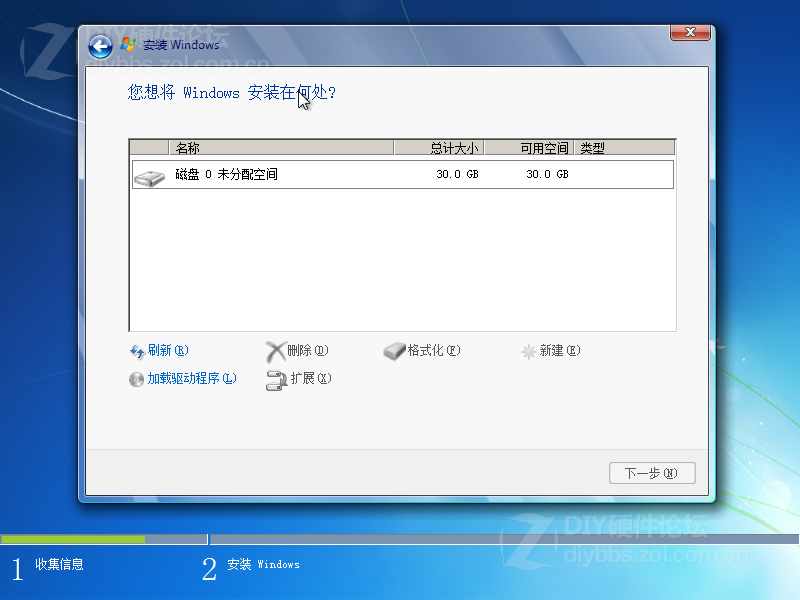
\includegraphics[width=5in]{1.png}
  \end{figure}
 \newpage

\item 输入diskpart后回车确定

 \begin{figure}[!ht]
  \centering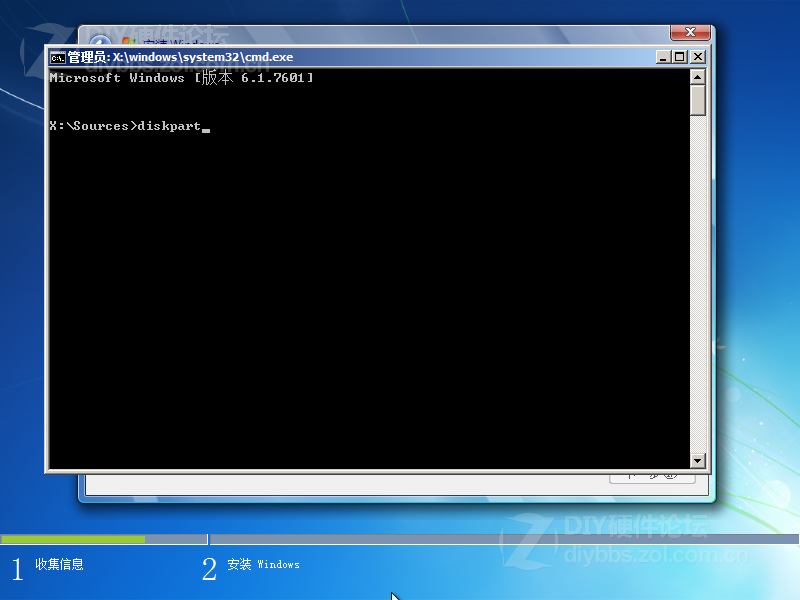
\includegraphics[width=5in]{2.png}
  \end{figure}\newpage

\item 输入list disk列出硬盘
  
 \begin{figure}[!ht]
  \centering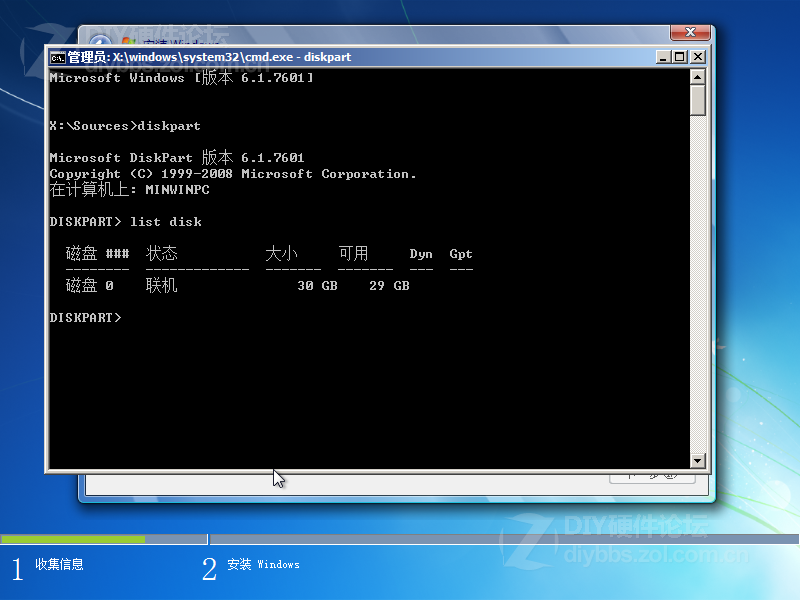
\includegraphics[width=5in]{3.png}
  \end{figure}\newpage

\item 如果你有多个硬盘,会列出0-N,这里只有一个,所以只有0,选择这个磁盘,输入:select disk 0

 \begin{figure}[!ht]
  \centering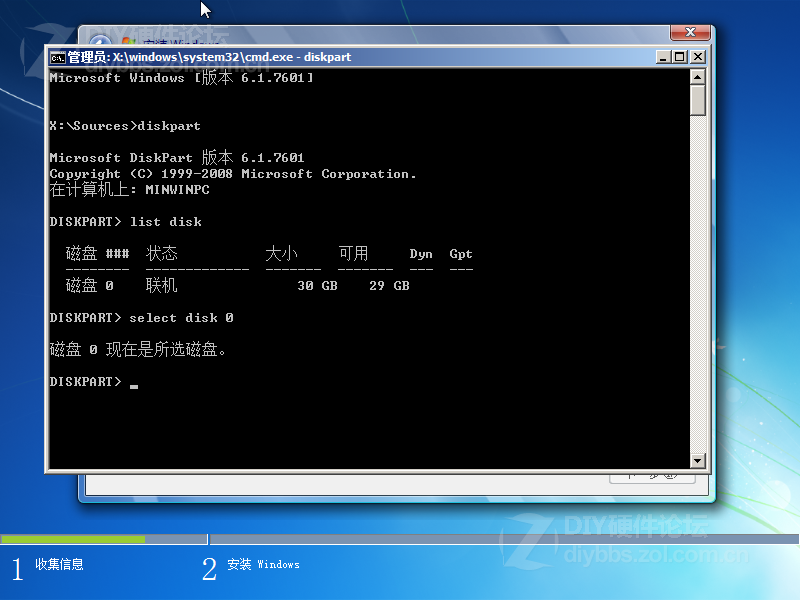
\includegraphics[width=5in]{4.png}
  \end{figure} \newpage

\item 如果你已经创建过了主分区,直接跳到下一步,如果没有创建主分区,那么输入create partition primary size=XXXX

这里XXX输入你想要创建的主分区的大小,如果这是第一个主分区,一般就是C盘了,这里是MB大小,如果输入1024MB=1G

在这里分主分区的好处就是,不会出现系统保留分区

 \begin{figure}[!ht]
  \centering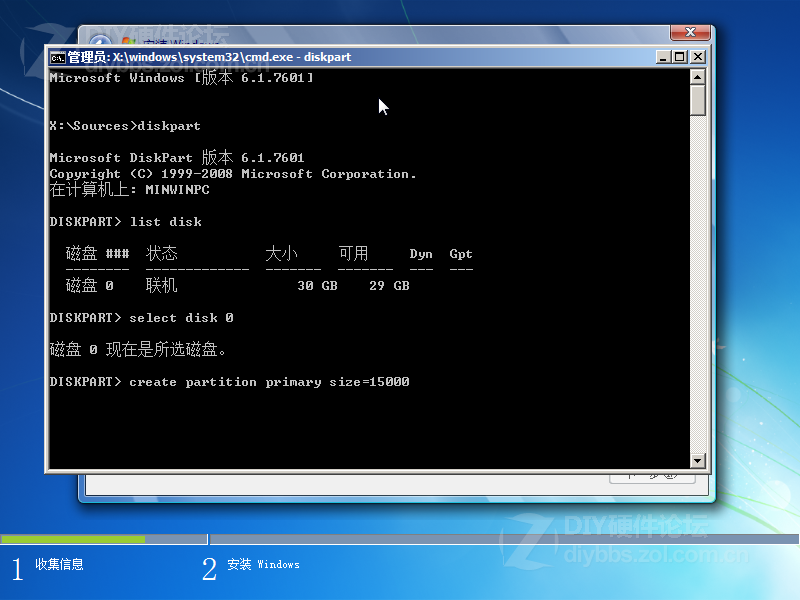
\includegraphics[width=5in]{5.png}
  \end{figure} \newpage

\item 下面是创建扩展分区输入命令:create partition extended,输入这个命令,所以剩余的未被分区的硬盘,都将变成扩展分区,如果只想分出一部分,可以参考步骤5,在create partition extended后面加上size=XXXX,如create partition extended size=100000

 \begin{figure}[!ht]
  \centering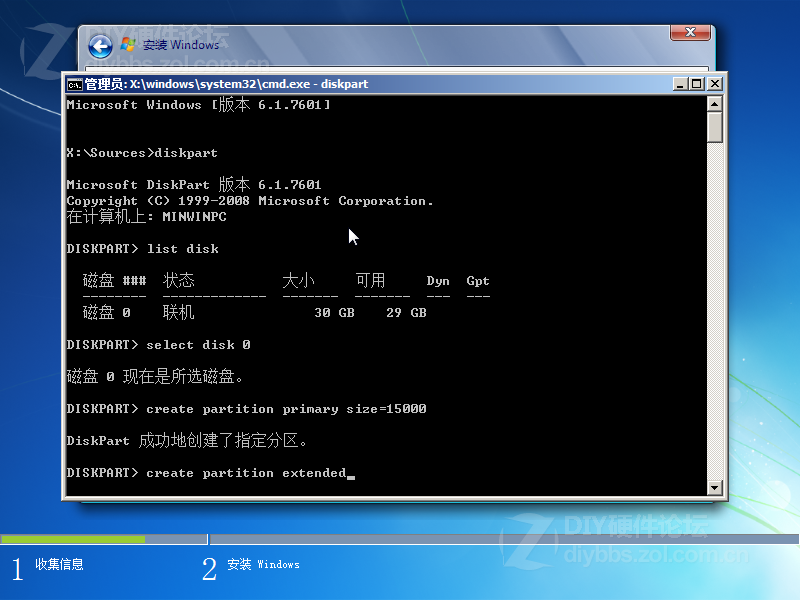
\includegraphics[width=5in]{6.png}
  \end{figure}\newpage

\item 然后关闭刚才的cmd,出现下面的图,刚才分的区没出现?不用担心,点一下刷新
 \begin{figure}[!ht]
  \centering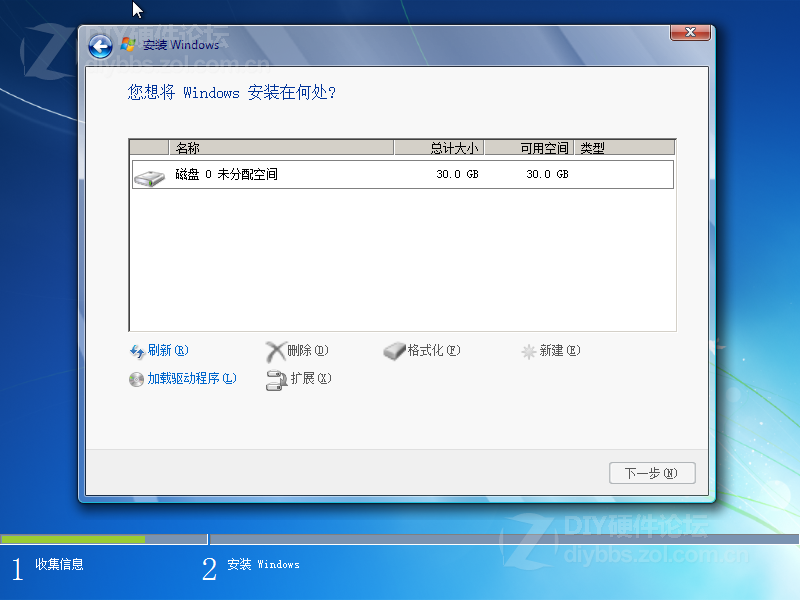
\includegraphics[width=5in]{7.png}
  \end{figure}\newpage

\item 现在已经出现刚才分的主分区和扩展分区了,但是扩展分区是不能直接用的,必须再扩展分区下面分出逻辑分区才可以,选中扩展分区,然后点新建

 \begin{figure}[!ht]
  \centering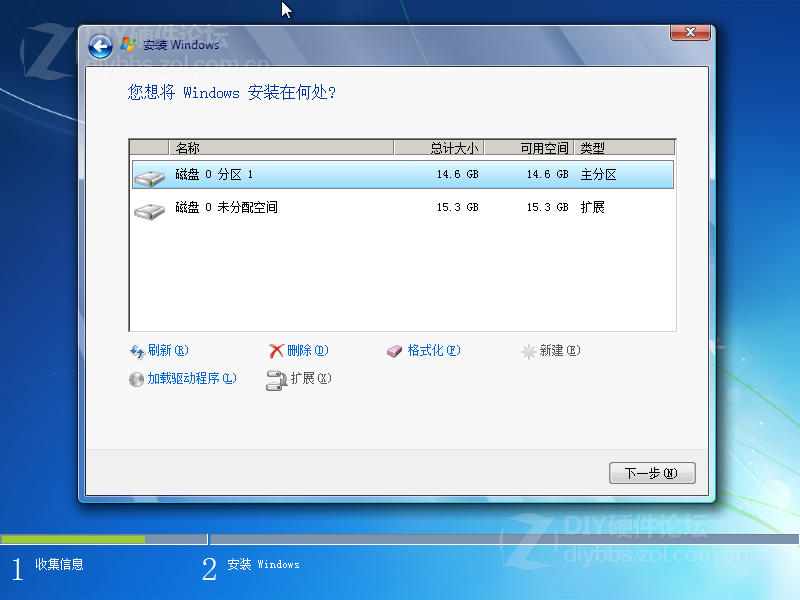
\includegraphics[width=5in]{8.png}
  \end{figure}\newpage

\item 输入你想建立一个多大的分区,大小不能超过扩展分区的总容量

\begin{figure}[!ht]
  \centering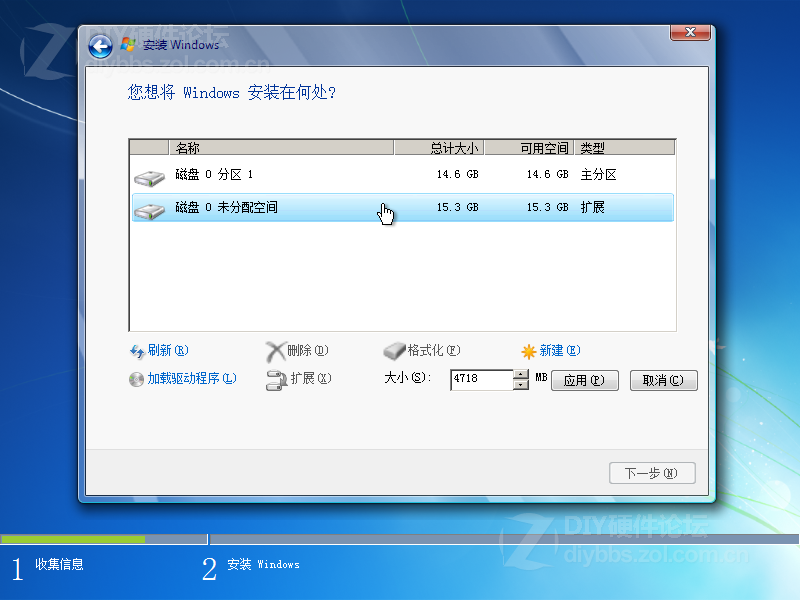
\includegraphics[width=5in]{9.png}
  \end{figure}\newpage

\item 如下图,那个15.3GB的扩展分区,被我分出了4个逻辑分区

\begin{figure}[!ht]
  \centering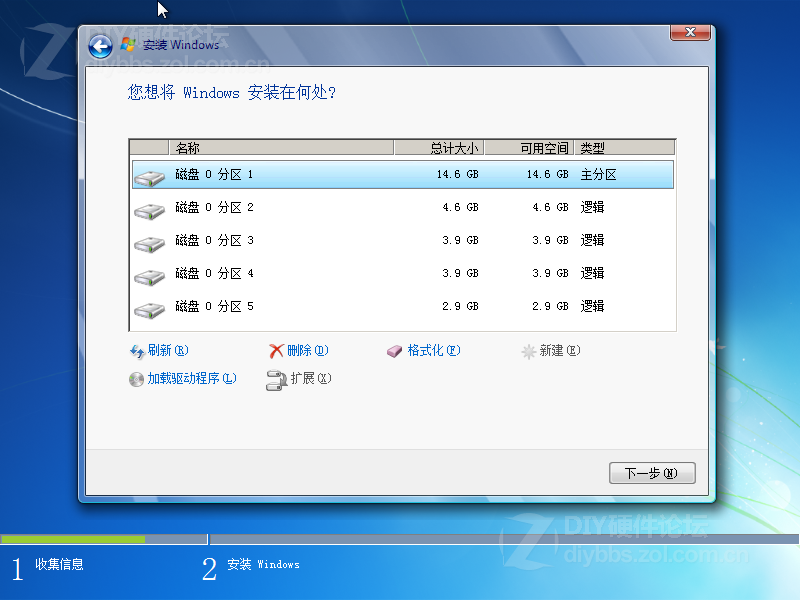
\includegraphics[width=5in]{10.png}
  \end{figure}\newpage

\end{enumerate}



\end{document}
